\chapter{Elaboration of the design and implementation}
% ------------------------------------------------------------------------------
% Elaboration 20 pages. Details of the Dependency Analysis Plugin (DAP. Describe
% the DAP-DB and %DAP-INCQUERY solution too.
% ------------------------------------------------------------------------------


% ------------------------------------------------------------------------------
% MODULE: Bytecode analysis
% ------------------------------------------------------------------------------
\section{Server side}\label{sect:elabserver}


\subsection{Bytecode analyzer}\label{sect:bcanalyzer}
% Why
Before the system performs dependency analysis, it needs to extract the
necessary information from the source code.
% What
The bytecode analyzer module takes the input java binaries (in the form of jar
files) parses the contained class files with the help of Apache BCEL and maps it
into an object graph which can be effectively used during the dependency
processing.

% REDUNDANT,
% How
% \subsubsection{Anatomy of a Java binary}
% The Bytecode analyzer module takes a set of jars as an input. A jar file is
% essentially a zip file containing Java-related resources: resource files, binary
% class files and meta-information. Because the system has to discover
% dependencies between pure Java applications then no meta-information is used;
% the bytecode analyzer gets the information from the class files contained in the
% jars.
%  
% 
% % Describe the ConstantMethodRef/FieldRef/Class/String in more details?
% \autoref{fig:classfile.pdf} shows a simplified view how a single class
% file is built. This structure is precisely defined in the Java Runtime
% Specification. The class begins with a marker header followed by the part called
% \textit{constant pool} which contains the textual part of the code. It contains
% the i) constant strings ii) referenced methods and fields and iii) the names of
% the external classes. The Java virtual machine is only able to load a class file
% if all the referenced external classes are loaded.
% %\pic{classfile.pdf}{Internal structure of a class file}
% After the constant pool the access flags, the implemented interfaces and the
% field list are located in separate places.
% 
% % Describe the bytecode instructions?
% Afterwards comes the definition of the methods. It contains all the necessary
% information for the virtual machine to execute the methods: the resources to 
% allocate for the execution, the exception handlers and the bytecode itself. 
% 
% The big question is what information can be extracted from the jar/class files
% for the dependency analysis? The short answer is everything. The structure of a
% class file can be obtained one-by-one. The external references what we are
% looking for are also fairly easily to extract, because they are defined in the
% constant pool. The only challenging part to solve is to match, where exactly are
% the external resources are used in the bytecode itself.


\subsubsection{The analysis process}
The module extracts all necessary information from the class files by processing
them. The analysis is done via Apache BCEL to effectively parse the class file
and to obtain the necessary information via simple API calls.
\pic{bytecodeanal.pdf}{Steps of the bytecode analysis process}
\autoref{fig:bytecodeanal.pdf} shows the workflow of the analysis process and the
used information from the class files for each step.

\paragraph{Initialization}
The analysis starts with gathering the basic structure. This involves acquiring
the class' name, the name of the extended class and the implemented interfaces,
the defined fields and methods. This information is accessible out of the box
through the BCEL API.  

\paragraph{Gathering external references}
The second step is to acquire all external reference pointing outside of the
class files. For imported classes it is easy because this is what the
\code{ConstantClass} entries cover in the constant pool. For field and method
references, the implementations searches \code{ConstantFieldRef} and
\code{ConstantMethodRef} occurrences in the bytecode and saves all methods 
which uses them.

\paragraph{Conversion}
The next step is to convert the information into source format. This is
necessary because both the structure and the external references are presented
in a format which not readable nor could be easily queried by the users of the
data. For example the commonly used \code{println(String)} function has the
following binary format: \code{println(Ljava/lang/String;)V}. The implementation
transforms it into \\ 
\code{println(java.lang.String):void}.

% Somewhere it should be described that we don't deal with reflection, just
% static dependencies.
\paragraph{Filtering}
The final step is to filter  the gathered information. At this step we have to
consider that if we mapped all information then the gathered data would have a
comparable size with the binary repositories which is unacceptable when we have
to deal with thousands of jars. To resolve this, the implementation does
multiple cleanup steps. First it drops the private methods and fields, because
it is not explicitly accessible and by this no dependency would point them. The
other trick is to drop a subset of the external references. The
platform-provided elements are dropped (references pointing inside the
\code{java.*} package) and the ones which point inside the jar files. This is
reasonable because any IDE gives access this information through code traversal
capabilities. Of course this cleanup needs do be done after all class files are 
parsed in a jar file. 


\subsubsection{Extracted domain model}
The output of the analyzer is a Java domain metamodel shown on
\autoref{fig:domainmodelsimp.pdf}\picr{domainmodelsimp.pdf}{Classes of the
domain model used by the bytecode analyzer}. Because this model is used for the
dependency processing too the model has additional elements holding the
dependency references.

All element inherits from abstract \code{CodeElement} class which is a top-level
interface for handing the items of the model. The processed jar files are named
as \code{Product}s, because that's what it is: a software product. A product
contains several classes named \code{ApiClass} which store the class-level
properties. The required classes are stored in the \code{referencedClasses}
list. The classes contain some \code{Field}s and some \code{Method}s which both
have a -- source formatted -- signature and some access properties. The
\code{referencedFields} and the \code{referencedMethods} hold all the external
field and method references which are accessed or invoked in the bytecode of the
represented method.

With an instance of this domain model the dependency processing module is
capable of discovering the dependency relationships between certain parts of the
dependency.
 

% ------------------------------------------------------------------------------
% MODULE: Dependeney processor
% ------------------------------------------------------------------------------
\subsubsection{Dependency processor}
% Why
The bytecode analyzer gathers all structural elements and the textual references
of the dependencies. For resolving the references the dependency processor
component is responsible.

% What
To achieve this the processor takes the models of the jar files, compares the
contained references with the structure of the external jars. When a match is
found it means that there is a dependency between two elements and as a result
a dependency link is stored.

% How
\subsubsection{Discovered dependencies}
At CERN we decided to narrow down the search for basic
dependencies which could be extracted from the binary code without interpreting
what does a class really do. By this we could exactly define what information
will be accessible for the users. The following list contains the discovered
dependencies:
\begin{description}
\item[Class import] When a class uses \emph{any} part of an external class. 
Practically, this is a relationship between two classes when one class requires
the other to get loaded in the Java virtual machine. On a binary level it is 
expressed as a \code{ConstantClass} entry in the constant pool.  
\item[Inheritance] When a class inherits from another. This dependency type 
covers both the case when an interface is implemented and when a class is 
extended. 
\item[Method call] When a method calls an another method. Covers both static 
and non-static method calls.
\item[Method override] When a class extends from an another and the subclass 
has a method with a same signature which was already defined in the superclass.  
\item[Field access] When a method accesses or gives a value of a field defined 
in an external class.
\end{description}


\subsubsection{Two-pass discovery process}
The main objective here is to do the analysis on a large set of Java binaries
without having memory problems. If one loads all jars to the memory at the same
time, it will need an enormous size of memory which will go up if the input
number of the binaries increasing.

\picr{analization.pdf}{Sequence of the dependency discovery process}

\paragraph{Binary update processing}
\autoref{fig:analization.pdf} shows how the tool solves this issue. The process
starts with an update in the binary repository. The new, not yet analyzed
binaries are passed to the bytecode analyzer components which produces a model
for each jar files. These models are passed for the dependency processor which
stores the jar structure in the database. By doing this, the implementation
holds only one model in the memory, which implies that the memory requirement is
independent from the number of input binaries. Additionally only the structure
is pushed into the database, the references are considered as transient data.
This is necessary because the references may require a large amount of memory:
on average they took 60\% of the size of a class file and leaving them out
significantly reduces the required storage space.

\paragraph{Dependency reprocessing} 
After all jar's  structure is saved in the database, the process re-initiates
the bytecode analysis on every jars one-by-one and passes the models again to
the dependency processor. The processor now tries to execute certain queries on
the database for searching dependencies. For external references, it tries to
find the elements with the same fully qualified name, for inheritance it searches for
superclass in the database and for method override it looks for methods with
the same signature in the superclass. For every found element  a separate dependency
entry is saved at the end of the analysis of the active jar.

The result of the analysis is a database containing all  structural
and dependency information. The clients can execute queries on it to analyze the
relationships between certain elements in order to decide whether or not a
specific code could be changed.
 
 
\subsection{Storage engine} 
The dependency processing requires some database functionality to 
properly work. This is defined in the storage engine component.

Although, this component is defined by a single Java interface it comes with
important and complex responsibilities. First, it is an abstraction layer over
the concrete database implementation. Second, it provides transactional behavior
automatically to the database. 

\subsubsection{Interface}
The interface defines operations for two purposes: 
\begin{enumerate}
  \item store and retrieve the structure of a jar and the dependencies,
  \item search for items based on their names, and
  \item query incoming dependencies of an element.
\end{enumerate}

The usage of the first is easy the understand: if the analyze process starts it
has to be checked if the a jar is in the database and if not, it has to be
stored. The second in the list is part of the dependency processing. It is the
responsibility of the database component how to represent the data and thus,
finding references also belongs here. The last part covers the queries which are
initiated by the clients and the result is also provided by this module.

To make the domain model usable to store dependencies and make it work with the
same jar products with multiple versions the domain model was extended (see
\autoref{fig:domainmodelext.pdf}). \pic{domainmodelext.pdf}{Additions to the
domain model} Every element has a list of version numbers where they are
present. Also a \code{Dependency} class is added to effectively handle
dependencies between them.

\subsubsection{Implementations}
This database engine is just a specification how it should work. It has two
practical implementation: one which uses Oracle database and one which stores
the data in an EMF model. The Oracle database maps the entities into tables and
execute complex SQL queries in order to find the desired elements.

The EMF version is an in-memory implementation with an optional serialization
feature implemented. The EMF metamodel used for creating the model has the same
structure as the domain model (see \autoref{fig:domainmodelsimp.pdf} and
\autoref{fig:domainmodelext.pdf}).

% TODO: maybe the explanation of the two deps implementation would be fine to
% show here


\subsection{Elaboration of the example}\label{sect:elabex1}
After showing the details of the implementation, the current section highlights
certain parts through our running example described in \autoref{sect:spf}.
We will check how the individual components evaluate the example as an input and
how the users can utilize the provided information.

\paragraph{Repositories}
In our example the source and the binary
repository contains three pro\-jects, each of them holds one package from the
example. the name of the projects are service, client and impl, the name of 
the jars files respectively service.jar, client.jar and impl.jar. 
This will be the input for the bytecode processing.

\paragraph{Bytecode processing}
As 
the binary projects appear in the repository, they get discovered by the 
server process. 
The first step in the process is the bytecode analysis. In this phase the
structure and the reference of the dependencies are discovered from the
binaries. As of the structure the analyzer finds 3 projects, 8 classes 2 fields
and 19 methods which get stored in the database.
The methods are composed of the 12 defined methods, 6 constructor (from all
non-interface classes) and 1 static initializer (which comes from the Services
class as it gives a default value to a static field).

\paragraph{Dependency extraction}
The discovered dependencies are formatted and filtered in order not to have
internal or platform defined elements (dependencies pointing inside the
\code{java.*} package). For example, let's see the \code{BasicImplUtil} class'
\code{registerImplementation()} method.
\begin{tabl}
{External references of the BasicImplUtil.registerImplementation() method}
{extrefs}{|p{.37\linewidth}|p{.37\linewidth}|p{.2\linewidth}|}
\hline
	\textbf{Binary format}						&  
	\textbf{Source format} 						& 
	\textbf{Type} 								\\
\hline
	impl/BasicProvider  						&
	impl.BasicProvider 							&
	ConstClass 									\\
\hline
	service/Services/registerProvider 
	\mbox{(Ljava/lang/String;}
	\mbox{Lservice/Provider;)V} 				& 
	\mbox{service.Services.registerProvider}
	\mbox{(java.lang.String,}
	\mbox{service.Provider):void} 				&
	\mbox{Constant} \mbox{MethodRef} 			\\
\hline
\end{tabl}
The first one is a 
\code{ConstantMethodRef} type reference. During the analysis they are first converted into source format.
The first one is a class reference the second one is a method reference.
The references are formatted to source format as it is shown in the second column.
Now the first references is eliminated from the list, because it points inside the 
\code{impl} project. However the second one does not, so it remains at its place.  

The dependency processor takes the remaining dependencies from the elements and 
searches the database if there is one. In case of our method reference, the processor
finds that there is a \code{registerProvider()} method defined with the same exact 
signature signature in the database. Because the reference was stored on the called 
method list, the processor creates a new method call dependency starting from 
\code{impl.BasicImplUtil} targeting \code{Services.registerProvider()}.

\paragraph{Persistence}
At this point, the storage engine stores all the structure and the dependencies 
of the three products. The schema of the Oracle database implementation and the EMF
database was described in details previously.



% ------------------------------------------------------------------------------
% MODULE: Dependeney processor
% ------------------------------------------------------------------------------
\section{Client side}
\subsection{Dependency database synchronizer}
\label{sect:depdbsynch}

\subsubsection{Overview}
The Dependency database component is responsible for querying the server for
dependency information related to a selected element or elements. It loads the
part of the dependency data stored by the storage engine module through a
simple RMI interface and pushes it to the model queries component where the
result is evaluated.

The database synchronizer has two modes of operation: either it can load a compacted
representation of the entire dependency model or it can query the incoming
dependencies for just one single code element.
The single element query is the use-case where the user of the \ptool{} executes
direct queries by asking the incoming dependencies of one element in the
workspace. In this case, a simple RMI interface method is called where the
argument is the queried object (as an instance of an \code{ApiClass}, a \code{Method} or a
\code{Field} types from \autoref{fig:domainmodelsimp.pdf}. This argument is passed to
the server, which turns it into an SQL query or a search on the EMF model
(depending which back-end is loaded). The result is passed back as a collection
of \code{Dependency} instances. The result model is unattached by the model
queries component and gets instantly visualized in the UI component.

\subsubsection{Compacting models to balance resource usage with analysis precision}
The resource constraints of virtualized developer PCs at CERN implied that the
repository model has to be compacted. 
For letting the model queries component run real queries, this model has to load
a representation of the data stored by the database engine component. If it was
loaded one-by-one into an EMF model and passed to the client, then it would be
simply too big to load. The binary repository holds more than a thousand jars
just as latest production versions. The serialized EMF model equivalent is more
than 400 MiB in size. To load an EMF model this size, more than one GiB of
RAM is needed.

% Important details about the environment at CERN is that the developers usually
% do the development on dedicated virtual machines which have more privileges to
% access internal resources. The drawback is that usually a virtual machine has
% 1-2 GiB RAM total, so we cannot make an Eclipse plugin which consumes all
% remaining resources at once. Also EMF-IncQuery has a practical limitation as it
% can easily handle EMF instance models up to 100 MiB.

We can drop the unnecessary information or
merge certain data and structure to spare some space without introducing false
negative results. If we leave information the clients may end up false
conclusions as they for example see an empty incoming dependency set where
should be some.
While this compacting process results in result over-approximation (potentially
false-positive results), but in return lets the model queries component to do
fast model queries which are automatically updated every time the source code
has changed.

\picseventy{cp3model.pdf}{Compacted repository model}

\paragraph{Metamodel for compacted repository models}
The structure of the compacted EMF metamodel is shown on
\autoref{fig:cp3model.pdf}.
The first thing which was left out are most of the fields of the classes; only a
\code{name} field stores the textual representation of the code element. This is
reasonable because the dependency discovery is done on the server and we
navigate only on the dependency edges. The second thing is not explicitly
visible on the figure. The fully qualified name was trimmed into simple
names. It means that there is only one \code{Service} class for all products in
the repository and one \code{newService()} function. If there are more, than one
exists, then they are merged into one and also all dependencies becomes common.
This also comes with the change that the original one-to-many containment
relationships became many-to-many. The third compacting change is to drop the
signature of the methods, only the name has left. Here the same merging process happens.

\paragraph{Managing repository models on the client side}
This compacted repository model is loaded at start-up time and used till Eclipse
is closed. This is reasonable because the repository changes are considered as rare events: 
In the environment described in \autoref{sect:cerninf} only a few releases happen a day.

The compact model is small enough to load it into the memory: the serialized
representation of the entire CERN software infrastructure is around 70 MiB which
is considered small enough to work with.

% ------------------------------------------------------------------------------
% MODULE: Source code model synchronizer
% ------------------------------------------------------------------------------
\subsection{Source code model synchronizer}
% what
To make the repository model comparable with the state of the workspace the
source code model synchronizer generates an EMF model describing the elements
in the workspace and keeps it synchronized along every workspace modification.
Maintaining an EMF model lets the model queries component dynamically examine
the current state of the workspace without accessing the JDT API.

\subsubsection{Eclipse Java Model}
The objective of the Eclipse Java Development Tools \cite{JDT} is to provide a
feature-rich, integrated and extendable environment for editing Java source
code. It comes with incremental builder and rich and extensive tooling for Java
editing. Contributors can get all the necessary information about the state of the
workspace.

The state of the Java projects are exposed through an API called the \emph{Java
Model}. It is a complex yet intuitive set of Java interfaces which can be
traversed easily. Instead explaining what classes and interfaces are present in
this API, let's examine which API elements represents which Eclipse- and
Java-specific elements.
\begin{figure} 
        \centering
        \begin{subfigure}[b]{0.5\textwidth}
                \centering
                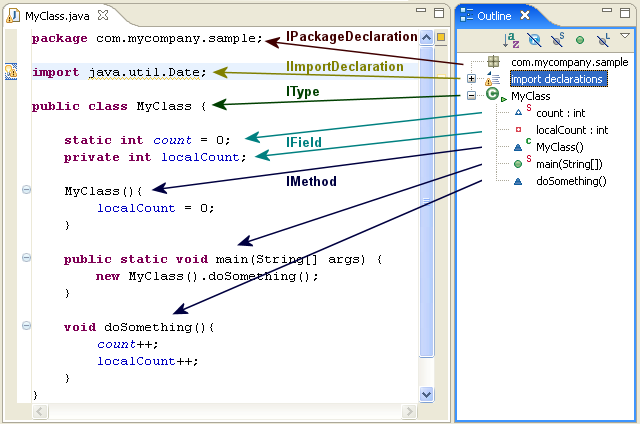
\includegraphics[width=\textwidth]{figures/javamodel2.png}
                \caption{Java Model elements from the source code}
                \label{fig:javamodel2.png}
        \end{subfigure}~
        \begin{subfigure}[b]{0.5\textwidth}
                \centering
                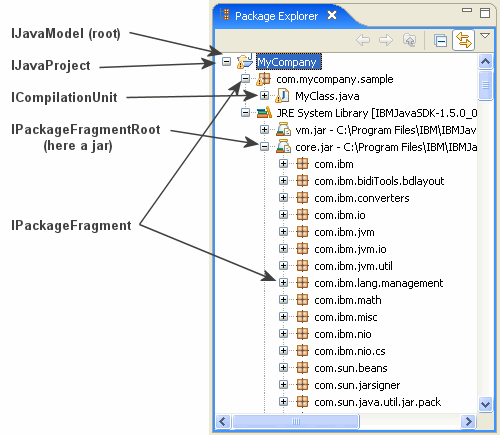
\includegraphics[width=\textwidth]{figures/javamodel1.png}
                \caption{Java Model elements from the navigator}
                \label{fig:javamodel1.png}
        \end{subfigure}
        \caption{Java Model elements}\label{fig:javamodel}
\end{figure}
\autoref{fig:javamodel} (which comes from JDT's documentation) shows these
relationships as the main elements of the Java model. Visible: literally every aspect 
is accessible from the defined projects down to the method level. As the Java Model 
is hierarchical the implementation simply traverses it to build the java model. 

The elements explained above is enough to create a model about the structure of
the Java projects. To add dependency information to this model, the JDT's search
feature comes into picture. With this the component is able to query the dependencies
for every structural element. 

\subsubsection{Generating EMF models from the Java model}
% structure and JDT
\picr{wsmodel.pdf}{EMF model storing the structure of the Java projects}
\autoref{fig:wsmodel.pdf} shows the EMF model which is extracted and maintained
from from the Java Model. It mostly mirrors the structure of the Java model's
interface structure. The key element is the \code{WNamedElement} which is common
superclass for all items. The \code{handler} property holds an identifier string
which uniquely identifies the represented Java Model object. To gain access to
the correspondent Java Model object, only the \code{JavaCore.create(String)} is
required.

\paragraph{Structural hierarchy}
The containment hierarchy starts form the lower right corner of the figure with
the \code{WProject} class which represents a Java project loaded into the
workspace. It contains \code{WPackageFragmentRoot} elements which represent the
source folders and the jar files on the classpath and has some Java packages as
children(as \code{WPackageFragment} instances). Under the Java packages there
are the \code{WCompilationUnit}s which are represent the java files and which
define some java types (\code{WType}). On the lowest level in the containment
hierarchy lie the methods and fields (\code{WMethod} and \code{WField}
instances).

\paragraph{Dependency hierarchy}
Just like in the repository model, here also the dependencies are defined upon
the common supertype, but here a \code{WDependency} has a two-way relationships
for both the source and the target part of the dependency relation. For one
\code{WNamedElement} the incoming and outgoing dependencies are directly
accessible. Again, the same dependency types are defined as before.

% root
The model has one common root, a \code{WWorkspace} instance which contains both
the structural elements and the dependencies.

\subsubsection{The model synchronization process}
% describe the process itself
\picr{sourcesync.pdf}{The maintenance process of the source code model}
\autoref{fig:sourcesync.pdf} shows how the process  of model building works. It
starts with mapping the entire workspace structure (projects, classes, etc.)
into the model. During the process the entire workspace is traversed. If it is 
done the components executes a dependency search for each relevant element 
utilizing JDT's integrated search engine. The found dependencies are associated 
with the proper model element.

\paragraph{Capturing local workspace changes}
When the initial model build is finished the next task is to subscribe for the
workspace changes. This can be done by registering a simple listener object with
the  \code{JavaCore.addElementChangedListener(IElementChangedListener)} static
method. With this every event related to the java editing is available. The
component only handles the events where the source files are changed; dealing
with working copy events would be too frequent and would contain some incoherent
data about the workspace. 
	
After the component is set up it waits for the modifications. If it happens, an
incremental model update fires, maps the related Java Model element to the EMF
model and modifies it accordingly. 

\paragraph{Processing local workspace changes}
The change notifications comes in a form of a hierarchical delta holder object.
It refers to an object, states if it was added, deleted, or changed and provides
the list of the affected children. For example if a Java class definition has
been deleted, the generated event contains a changed project down to the
container changed compilation unit which has a child delta pointing to the
deleted class.

\paragraph{Workspace content modifications}
The use-case when an element was added or deleted the model update is
straightforward. The event contains the reference of the modified item. It is
identified via the \code{handler} property. The result of the event is a
creation of a new element or removing an existing one along with all his
children and their dependencies.

\paragraph{Source file modifications}
If a modification happens in the source file it is also incrementally modified
but treated slightly differently. This is necessary because the delta
information doesn't provide usable information about what has changed below the
compilation unit.

\pic{sourceupdate.pdf}{Updating EMF workspace model when source code is modified}

This process is shown in \autoref{fig:sourceupdate.pdf}. The updater checks
which source file is modified and re-generates its EMF representation. The
generated small model is compared with the source of the model. If a new method
is added than it is merged into the old model. If an element is missing, it gets
deleted from the original model too. Dependencies are the same: any differences
are immediately pushed back to the original model. With this approach the EMF
representation of the workspace stays consistent and only local modifications
happen on the elements.

\paragraph{Generated model lifecycle}
When Eclipse closes, the model is stored on the disk in order not to regenerate
the entire model when on the next start-up. If no external modifications happen
than the model is loaded one-by-one which is faster than gathering all
structural and dependency information.

\subsection{Explicit queries}
\label{sect:elabexplicit}
The model queries components executes complex queries on the loaded models and
gives and exposes the result for  visualization. 

The UI components extends the Eclipse platform's user interface to provide
access to the dependency information and to show the results in an integrated
way. The Eclipse views utilize JFace~\cite{JFace}, more precisely JFace tree
viewers to present the information. Using JFace has two advantages: displaying
the data is not bound to the original structure of the input and EMF has tight
integration to JFace out of the box.

\picfifty{jface.pdf}{Displaying data with JFace}

\autoref{fig:jface.pdf} shows a simplified view how the data is presented in
JFace viewers. Originally the results are a simple net of objects. In the first
step it is restructured into a into an internal tree structure. This tree is the
input content for the display. To make JFace understand  the structure of this
data, a data adapter is loaded (through Eclipse platform service registration).
With both the content and the description how the data should be displayed JFace
automatically shows the results and provides convenience functions such as tree
folding, selection service, etc. 

\paragraph{UI integration for explicit query results} 
The first part is the UI extension for explicit queries. The Java source code
editor gets an new element in the context menu with the label ''Show Incoming
Dependencies''. The developer selects any code element in the source code (he
can point to a class, a field or a method) right clicks on it and chooses this
menu element. The initiated action first resolves the selected element and tries
to get a fully qualified name of it. If it is successful the query is sent to
the server side for evaluation. After the result of the query is obtained, the 
result is pushed into an Eclipse view.

Let's see how the developer checks the incoming dependencies through the
explicit queries.
\pic{incdeps.png}{Execute explicit queries from the source code editor}
\autoref{fig:incdeps.png} shows the context menu contribution for initiating an
explicit query. The query takes a few seconds to respond. The results are shown
in the viewer like on \autoref{fig:results.png}.
\picr{results.png}{Result of explicit queries}


\subsection{On-the-fly model queries}

The main functional motivation for implementing client-side queries is to
support pre-release comparison between the local source projects in the
workspace and the last released state contained in the server-side database.
Additionally, the goal is to provide on-the-fly query evaluation so that the
feedback from dependency analysis can instantly be displayed to developers as
they are making changes to the source code, to speed up the development work.

To achieve this, the system first loads the model of the repository and the 
model of the current workspace, loads them into the EMF-IncQuery engine, 
and initiates the queries and exposes the results on an API which also updates
the dependency information dynamically.
 
\subsubsection{Query specifications based on graph patterns}
The queries are developed with EMF-IncQuery's own query
language~\cite{icmt2011}. This language is used to express certain patterns over
EMF models. You can think about it as a regular expression over an object-model.
To highlight this, let's see an example of a pattern expressed with this
language which matches on all Java files and all defined types in it from the
workspace model (see \autoref{fig:wsmodel.pdf}).
\begin{lstlisting}
package example

import "http://inf.mit.bme.hu/donat/incquery-deps/wsmodel"

pattern typesInJavaFiles(cu : WCompilationUnit, t : WType) = {
	WCompilationUnit(cu);
	WType(t);
	WCompilationUnit.types(cu, t);
}
\end{lstlisting}

The import declaration loads the EMF metamodel. The pattern signature
contains a name and a parameter list. Here the parameters define the result as
the found/matched items from the input model. 

The body of the pattern starts with two type constraints. This can be translated
as ''match only on the elements which have the \code{WCompilationUnit} type for
the \code{cu} variable and match the \code{WType} object for the \code{t}
variable''. Alone this would list all compilation units and all types as a
result in all possible combinations, just like in SQL when one select data from
two different tables at once without joining them. The third statements is the
connects the result items together. It can be translated as ''match only the on
the objects  where the \code{cu} variable refers the \code{t} as a contained
type''. Expression power of the pattern language is much bigger; for complete
reference check the documentation site \cite{EMFIncQuery}.

\paragraph{Developing model queries}
The usage of the queries takes multiple steps as shown in \autoref{fig:incquerydev.pdf}.
\picr{incquerydev.pdf}{Development of EMF-IncQuery queries} 
First, the queries are defined with the query language. The tooling takes the queries 
and automatically generates source code from the queries. With this there is no need 
for manually using the pattern definition part of the EMF-IncQuery engine. The generated
source code along with the engine exposes a simple interface for registering the
queries and getting back the results when needed. The only manual coding takes place
at the last part on load-time, when it has to be specified manually which queries 
should be evaluated. 

\paragraph{Integrating queries at runtime}  
The generated code contains a factory service which registers the query in the
engine. The query is represented as a \code{Matcher} object in the generated
code which gives back the results through the \code{Matcher.getAllMatches()}
method. The result is represented by \code{Match} instances which hold the result 
and all the necessary information to make it usable.

\subsubsection{Query definitions}
The following list enumerates all the  queries developed for the dependency
analysis.
\begin{description}	
\item[Join queries]
In order to compare the workspace with the repository it is necessary to find 
the correspondent element in the two model. The join queries are basic patterns 
which joins the projects, classes, fields and methods in the models. The result
of the queries are all the found elements which are the input for the queries 
below. 
\item[Workspace changes] These queries discover the differences between the 
workspace and the repository. The results are the projects, classes, methods
and fields added or removed from the source code.   
\item[Incoming dependencies] For every source code loaded in the Eclipse these
queries shows all elements depending  on them. All incoming dependencies for 
all classes methods and fields are the result of these queries. Also the type
of the dependency is available. 
\item[Outgoing dependencies] The queries in this category can be highlighted 
with the following: If a dependency exists in the workspace it should
exist in the repository too. If the workspace changes and the dependencies change
it can be source of the problem.  By checking the changed outgoing dependencies
which start form the selected items the developer can analyze it.
\item[Commit impact] This list contains queries which are the combination of 
the workspace changes and incoming dependencies category. They show the incoming
dependencies of items which have changed in the workspace. The result is the
impact which a possible release would cause.  One use-case is to show the
incoming dependencies of the deleted elements. Another can be inheritance on
the classes where a method is added.
\end{description}


\paragraph{Detailed elaboration}
One of the implemented queries is the one which retrieves the incoming method call 
dependencies from the model. The entire definition of this query is the following. 
\begin{lstlisting}[caption=Elements of the incoming method call dependency query,label=patternex]
private pattern joinProjects(repoProject : CP3Project, wsProject : WProject) = {
	CP3Project.name(repoProject, commonName);
	WProject.name(wsProject, commonName);
}

private pattern joinMethods(repoMethod : CP3Method, wsMethod : WMethod) = {
	CP3Project.classes.methods(repoProject, repoMethod);
	WProject.packageFragmentRoots.packageFragments.compilationUnits.types.
		methods(wsProject, wsMethod);
	find joinProjects(repoProject, wsProject);
	CP3Method.name(repoMethod, commonName);
	WMethod.name(wsMethod, commonName);
}

pattern incomingMethodCalls(wsTarget : WMethod, repoSource : CP3Method) = {
	find joinMethods(repoTarget, wsTarget);
	CP3Dep.from(dependency, repoSource);
	CP3Dep.to(dependency, repoTarget);
	CP3Dep.type(dependency, 1);
}
\end{lstlisting}

The first \code{joinProjects} query takes the projects from the workspace
instance model and connects them to the equivalent element in the compacted
repository instance model This join operation is based on the common \code{name}
property.

The \code{joinMethods} query does a similar thing, but in this case the methods
are joined together. The first two instructions gathers the container projects'
reference. The third instruction calls the \code{joinProjects} query, so the 
results are filtered to only to the elements which exist both in the workspace
and in the repository instance model. The methods itself also joined by 
checking the common \code{name} property.

The last \code{incomingMethodCalls} query returns the required results. It lists
the methods present in the compacted workspace instance model and its incoming
dependency elements in pairs. To find them, first the \code{joinMethods} query
is executed. Then it filters to all the elements which are pointed by a
dependency instance. Note that \code{repoSource} argument is bound to the
repository dependency object.

On start-up these queries are registered and accessible outside via a simple API.
The UI components use this API to access the dependency information and show the
current state in different views.

The complete source code for all the queries is available in \autoref{examplequeries}.


\subsection{Elaboration of the example - continued}\label{sect:elabex2}
To continue our example, we will examine the view of the developer who knows
only about his own \code{service} project. If the \ptool{} is  installed in his
Eclipse, the EMF model -- shown on \autoref{fig:wsmodel.png}
\picr{wsmodel.png}{Workspace model containing Service package from the example}
-- is built and synchronized automatically. On the figure we can see, that the
structure of the project (left) corresponds to the content of the EMF model
(right). In the model view, you can also see that the in-project dependency
relationships are also registered.

Because the \code{client} and the \code{impl} projects have references to the
\code{service} project, both of them are loaded to the repository model. It has all the
element but with the compacted version, so no fully qualified names. But because
there is no overlapping names between the classes and method than the compacted
model does not introduce false-positive results.


\subsubsection{The compacted model}
The compacted version of the repository instance model (produced by the
dependency database synchronizer) contains all the three projects from the
repository. Part of the model is shown on
\autoref{fig:cp3modelinstance.pdf}.\picr{cp3modelinstance.pdf}{Elements of the
compacted instance model} 

The structure contains the same projects and the same
classes as the original model, however the following information is eliminated.
\begin{itemize}
  \item The class objects has only their simple name left, the fully qualified name is left out.
There is no overlapping classes but they would have merged together if
there was any. Here the \code{client.Service} instance has only the name \code{Service}.
  \item The method signature was trimmed down int their names. All methods have only their 
name section of the signature, the parameter list, and the return value are dumped.    
The object representing the \code{service.Service.serviceB()} method contains only the \code{serviceB}
formation and has the reference on its container. 
  \item The only visible dependency on the figure points to the same elements as before.
  It defines a method call dependency which starts from the object representing the \code{client.Main.main()} method.
\end{itemize}


\picr{patternresults.pdf}{Pattern matching on the example}

\subsubsection{On-the-fly model query results}
After the compacted  model and the workspace model is loaded the model and the
EMF-IncQuery is initialized, the results of the pattern queries can retrieved
any time. The pattern matching strategy for the query described in \autoref{patternex} is
shown on \autoref{fig:patternresults.pdf}.

The pattern finds, that the \code{serviceB} method object from the workspace has
a counterpart in the repository: They have the same name and their container
project have also the same name (the project object are not shown). Then the
query finds, that there is a dependency which point on the \code{serviceB}
object at the repository as the target of a method call dependency. Because
these requirements are satisfied, The source of the dependency (the \code{main}
method) from the repository model and the \code{serviceB} method object from the
workspace are returned (elements with the red border).
 
The query was evaluated with the sample data in EMF-IncQuery's UI tooling. The
results are on \autoref{fig:modelqueryresult.png}.
\picr{modelqueryresult.png}{Result of the incoming method call dependency query}
This figure shows that the evaluation gave back the same exact results as it was
described on \autoref{fig:patternresults.pdf}.

In this example a dependency was found. In this case the developer 
has to decide whether he will maintain backward compatibility or he notifies the
maintainer of the \code{client} project that the API will break soon. If he tried
to modify the \code{serviceA()} method, we would have seen that there are no incoming
dependencies. It means that the developer can break the signature of the method as
he wishes. 






